\section{I/O Systems}

\paragraph{Device Management --- Objectives}
\begin{itemize}
  \item \textbf{Abstraction} from details of physical devices
  \item \textbf{Uniform naming} that does not depend on hardware details
  \item \textbf{Serialization} of I/O operations by concurrent applications
  \item \textbf{Protection} of standard-devices against unauthorized accesses
  \item \textbf{Buffering} if data from/to device cannot be stored in final destination
  \item \textbf{Error handling} of sporadic device errors
  \item \textbf{Virtualizing} physical devices via memory + time multiplexing
\end{itemize}

\paragraph{Device Management --- Techniques}
\begin{itemize}
  \item \textbf{Programmed I/O}:
  \begin{itemize}
    \item thread is busy-waiting for I/O operation to complete $ \to $ CPU cannot be used elsewhere 
    \item kernel is \emph{polling} state of I/O device (command-ready, busy, error)
  \end{itemize}
  \item \textbf{Interrupt-driven I/O}:
  \begin{itemize}
    \item I/O command is issued 
    \item processor continues executing instructions 
    \item I/O device sends interrupt when command is done
  \end{itemize}
  \begin{figure}[h]\centering\label{InterruptIO}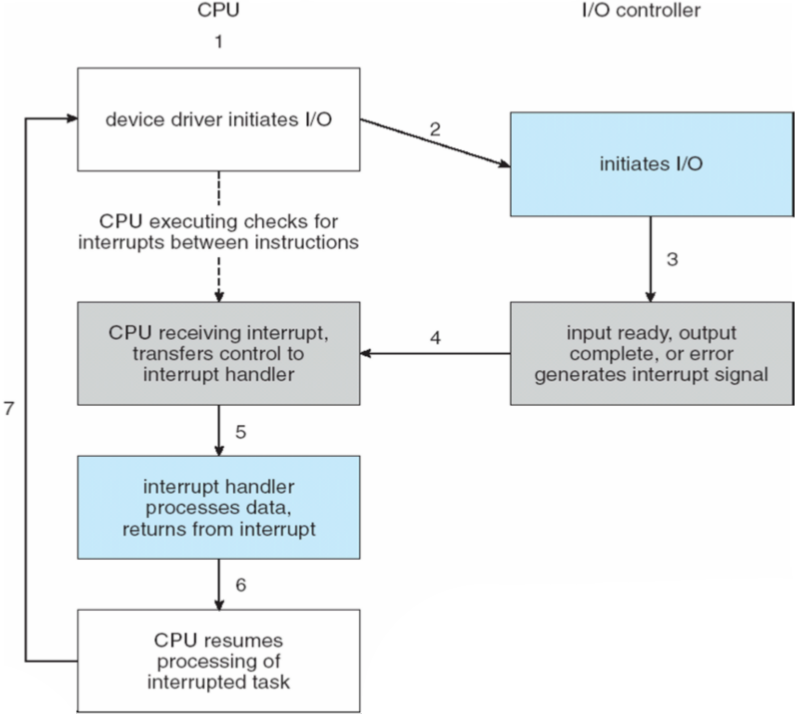
\includegraphics[width=0.33\textwidth]{InterruptIO}\end{figure}
  \item \textbf{Direct Memory Access} (DMA):
  \begin{itemize}
    \item DMA module controls exchange of data between main memory and I/O device 
    \item processor interrupted after entire block has been transferred 
    \item[$ \to $] bypasses CPU to transfer data directly between I/O device and memory
  \end{itemize}
  \begin{figure}[h]\centering\label{DMA}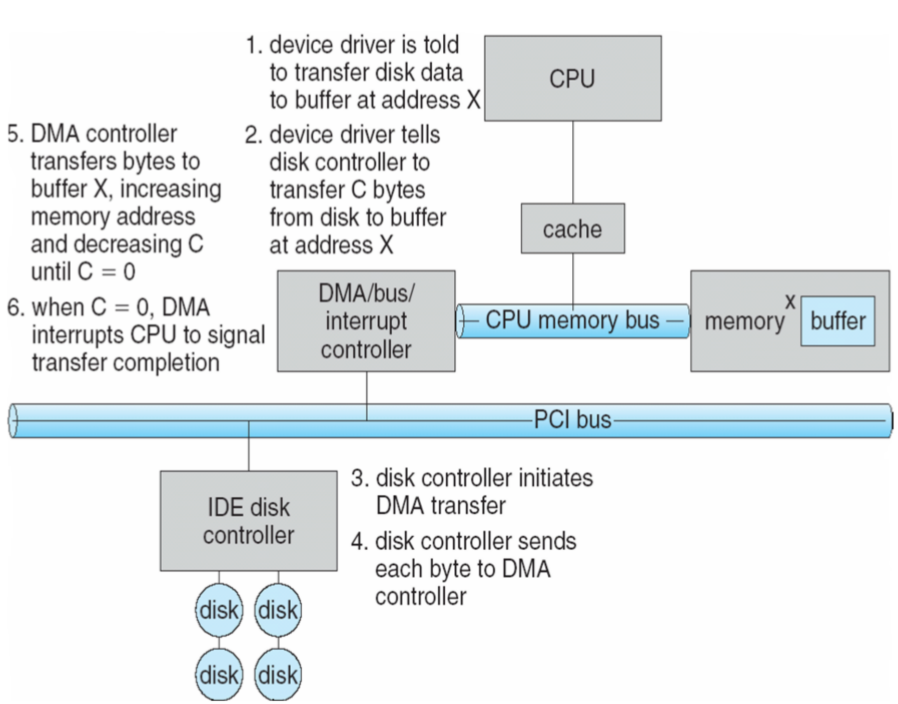
\includegraphics[width=0.33\textwidth]{DMA}\end{figure}
\end{itemize}

\paragraph{Kernel I/O Subsystem}
\begin{itemize}
  \item \textbf{Scheduling}: order I/O requests in per-device queues
  \item \textbf{Buffering}: store data in memory while transferring between devices
  \item \textbf{Error handling}: recover from read/availability/write errors
  \item \textbf{Protection}: protect from accidental/purposeful disruptions
  \item \textbf{Spooling}: hold output to device if device is slow (e.g., printer)
  \item \textbf{Reservation}: provide exclusive access for process
\end{itemize}

\paragraph{Device Drivers}
\begin{itemize}
  \item \textbf{Jobs}:
  \begin{itemize}
    \item \emph{translate} user request through device-independent standard interface 
    \item \emph{initialize} hardware at boot time 
    \item \emph{shut down} hardware
  \end{itemize}
\end{itemize}

\paragraph{Device Buffering}
\begin{itemize}
  \item \textbf{Reasons}:
  \begin{itemize}
    \item without buffering threads must wait for I/O to complete before proceeding 
    \item pages must remain in main memory during physical I/O
  \end{itemize}
  \item \textbf{Version 1 --- block-oriented}:
  \begin{itemize}
    \item information is stored in fixed-size blocks 
    \item transfers are made a block at a time 
    \item used for disks/tapes
  \end{itemize}
  \item \textbf{Version 2 --- stream-oriented}:
  \begin{itemize}
    \item transfer information as byte stream 
    \item used for keyboard, terminals, \dots (most things that is not secondary storage)
  \end{itemize}
\end{itemize}

\paragraph{Buffering --- User level}
\begin{itemize}
  \item \textbf{Principle}: task specifies memory buffer where incoming data is placed
  \item \textbf{Issues}:
  \begin{itemize}
    \item what happens if buffer is currently paged out to disk? $ \to $ data loss 
    \item additional problems with writing? $ \to $ when is buffer available for re-use?
  \end{itemize}
\end{itemize}

\paragraph{Buffering --- Single}
\begin{itemize}
  \item \textbf{Principle}: user process can process one data block while next block is read in
  \item \textbf{Swapping}: can occur since input is taking place in system memory, not user memory
  \item \textbf{Stream-oriented}: buffer = input line, carriage return signals end of line
  \item \textbf{Block-oriented}:
  \begin{itemize}
    \item input transfers made to \emph{system buffer} 
    \item buffer moved to \emph{user space} when needed 
    \item another block read into system buffer
  \end{itemize}
\end{itemize}

\paragraph{Buffering --- Double}
\begin{itemize}
  \item \textbf{Principle}: use 2 system buffers instead of 1 (per user process)
  \item user process can write/read from one buffer while OS empties/fills other buffer
\end{itemize}

\paragraph{Buffering --- Circular}
\begin{itemize}
  \item \textbf{Problem}: double buffer insufficient for high-burst traffic situations: 
  \begin{itemize}
    \item many writes between long periods of computations 
    \item long computation periods while receiving data 
    \item might want to read ahead more than just single block from disk
  \end{itemize}
\end{itemize}